\documentclass[8pt,aspectratio=169]{beamer}
\usetheme{Madrid}
\usepackage{graphicx}
\usepackage{booktabs}
\usepackage{adjustbox}
\usepackage{multicol}
\usepackage{amsmath}
\usepackage{amssymb}
\usepackage{listings}
\usepackage{xcolor}

% Color definitions
\definecolor{mlblue}{RGB}{0,102,204}
\definecolor{mlpurple}{RGB}{51,51,178}
\definecolor{mllavender}{RGB}{173,173,224}
\definecolor{mllavender2}{RGB}{193,193,232}
\definecolor{mllavender3}{RGB}{204,204,235}
\definecolor{mllavender4}{RGB}{214,214,239}
\definecolor{mlorange}{RGB}{255, 127, 14}
\definecolor{mlgreen}{RGB}{44, 160, 44}
\definecolor{mlred}{RGB}{214, 39, 40}
\definecolor{mlgray}{RGB}{127, 127, 127}

% Additional colors for template compatibility
\definecolor{lightgray}{RGB}{240, 240, 240}
\definecolor{midgray}{RGB}{180, 180, 180}

% Solidity colors
\definecolor{solkeyword}{RGB}{0,102,153}
\definecolor{solstring}{RGB}{163,21,21}
\definecolor{solcomment}{RGB}{0,128,0}
\definecolor{solnumber}{RGB}{0,128,128}

% Solidity language definition
\lstdefinelanguage{Solidity}{
  keywords={pragma, solidity, contract, function, public, private, external, internal, view, pure, payable, returns, return, if, else, for, while, mapping, address, uint, uint256, int, string, bool, bytes, bytes32, event, emit, modifier, require, constructor, memory, storage, calldata, msg, sender, value, this, new, delete, true, false},
  keywordstyle=\color{solkeyword}\bfseries,
  sensitive=true,
  comment=[l]{//},
  morecomment=[s]{/*}{*/},
  commentstyle=\color{solcomment}\ttfamily,
  stringstyle=\color{solstring}\ttfamily,
  morestring=[b]',
  morestring=[b]"
}

% Apply custom colors to Madrid theme
\setbeamercolor{palette primary}{bg=mllavender3,fg=mlpurple}
\setbeamercolor{palette secondary}{bg=mllavender2,fg=mlpurple}
\setbeamercolor{palette tertiary}{bg=mllavender,fg=white}
\setbeamercolor{palette quaternary}{bg=mlpurple,fg=white}
\setbeamercolor{structure}{fg=mlpurple}
\setbeamercolor{section in toc}{fg=mlpurple}
\setbeamercolor{subsection in toc}{fg=mlblue}
\setbeamercolor{title}{fg=mlpurple}
\setbeamercolor{frametitle}{fg=mlpurple,bg=mllavender3}
\setbeamercolor{block title}{bg=mllavender2,fg=mlpurple}
\setbeamercolor{block body}{bg=mllavender4,fg=black}

\setbeamertemplate{navigation symbols}{}
\setbeamertemplate{itemize items}[circle]
\setbeamertemplate{enumerate items}[default]
\setbeamersize{text margin left=5mm,text margin right=5mm}

\newcommand{\bottomnote}[1]{%
\vfill
\vspace{-2mm}
\textcolor{mllavender2}{\rule{\textwidth}{0.4pt}}
\vspace{1mm}
\footnotesize
\textbf{#1}
}

% TikZ and pgfplots packages
\usepackage{tikz}
\usepackage{pgfplots}
\pgfplotsset{compat=1.18}
\usetikzlibrary{arrows.meta, positioning, shapes.geometric, shapes.symbols, calc, decorations.pathmorphing, mindmap}

\title{ERC-20 Token Creation: A Visual Introduction}
\subtitle{Standalone Mini-Lecture}
\author{Prof.~Dr.~Joerg Osterrieder}
\institute{University Lecture Series}
\date{\today}
\begin{document}

% ==================== FRAME 1: TITLE ====================
\begin{frame}[plain]
\vspace{2cm}
\begin{center}
{\Huge\color{mlpurple} ERC-20 Token Creation}\\[0.4cm]
{\Large\color{mlblue} A Visual Introduction}\\[0.3cm]
{\normalsize Standalone Mini-Lecture}\\[0.3cm]
\textcolor{mlgray}{\rule{6cm}{0.4pt}}\\[0.3cm]
{\small\itshape ``Your own money --- with rules you write''}\\[1.5cm]
{\normalsize Prof.~Dr.~Joerg Osterrieder}\\[0.2cm]
{\small University Lecture Series}\\[0.2cm]
{\small \today}
\end{center}
\end{frame}

% ==================== FRAME 2: THE CUSTOM CURRENCY PROBLEM (Comic Strip 1) ====================
\begin{frame}{The Custom Currency Problem}
\begin{center}
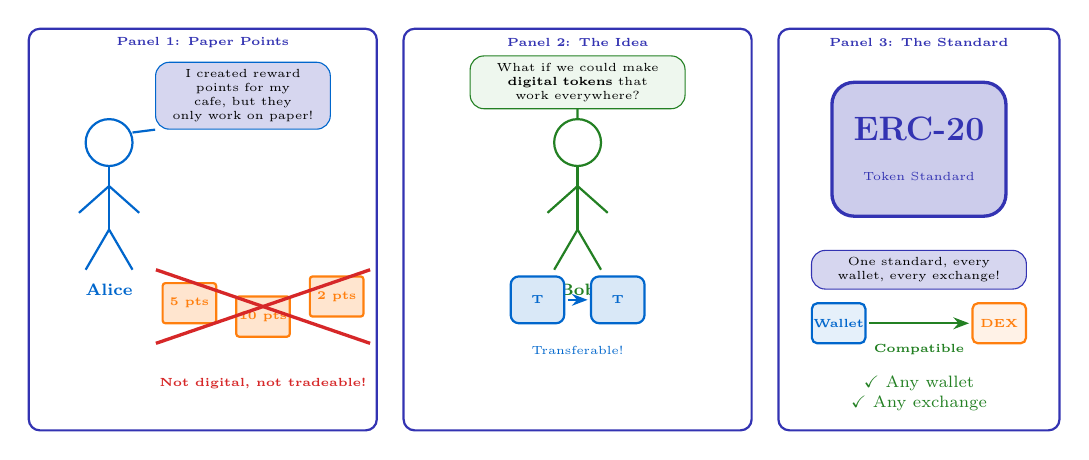
\begin{tikzpicture}[scale=0.85, every node/.style={transform shape}]

% --- Panel 1: Alice's paper reward points ---
\draw[mlpurple, thick, rounded corners=4pt] (-7.2,-2.8) rectangle (-2.0,3.2);
\node[font=\tiny\bfseries, mlpurple] at (-4.6,3.0) {Panel 1: Paper Points};

% Alice stick figure
\draw[mlblue, thick] (-6.0,1.5) circle (0.35);
\draw[mlblue, thick] (-6.0,1.15) -- (-6.0,0.2);
\draw[mlblue, thick] (-6.0,0.85) -- (-6.45,0.45);
\draw[mlblue, thick] (-6.0,0.85) -- (-5.55,0.45);
\draw[mlblue, thick] (-6.0,0.2) -- (-6.35,-0.4);
\draw[mlblue, thick] (-6.0,0.2) -- (-5.65,-0.4);
\node[font=\scriptsize\bfseries, mlblue] at (-6.0,-0.7) {Alice};

% Alice speech bubble
\node[draw=mlblue, fill=mllavender4, rounded corners=5pt, font=\tiny,
      text width=2.4cm, align=center, inner sep=3pt]
      (alice-bubble1) at (-4.0,2.2) {I created reward points for my cafe, but they only work on paper!};
\draw[mlblue, thick] (-5.65,1.65) -- (alice-bubble1.south west);

% Paper cards (scattered)
\draw[mlorange, thick, fill=mlorange!20, rounded corners=1pt] (-5.2,-1.2) rectangle (-4.4,-0.6);
\node[font=\tiny\bfseries, mlorange] at (-4.8,-0.9) {5 pts};
\draw[mlorange, thick, fill=mlorange!20, rounded corners=1pt] (-4.1,-1.4) rectangle (-3.3,-0.8);
\node[font=\tiny\bfseries, mlorange] at (-3.7,-1.1) {10 pts};
\draw[mlorange, thick, fill=mlorange!20, rounded corners=1pt] (-3.0,-1.1) rectangle (-2.2,-0.5);
\node[font=\tiny\bfseries, mlorange] at (-2.6,-0.8) {2 pts};

% Red X over paper cards
\draw[mlred, very thick] (-5.3,-1.5) -- (-2.1,-0.4);
\draw[mlred, very thick] (-2.1,-1.5) -- (-5.3,-0.4);
\node[font=\tiny\bfseries, mlred] at (-3.7,-2.1) {Not digital, not tradeable!};

% --- Panel 2: Bob's idea ---
\draw[mlpurple, thick, rounded corners=4pt] (-1.6,-2.8) rectangle (3.6,3.2);
\node[font=\tiny\bfseries, mlpurple] at (1.0,3.0) {Panel 2: The Idea};

% Bob stick figure
\draw[mlgreen!80!black, thick] (1.0,1.5) circle (0.35);
\draw[mlgreen!80!black, thick] (1.0,1.15) -- (1.0,0.2);
\draw[mlgreen!80!black, thick] (1.0,0.85) -- (0.55,0.45);
\draw[mlgreen!80!black, thick] (1.0,0.85) -- (1.45,0.45);
\draw[mlgreen!80!black, thick] (1.0,0.2) -- (0.65,-0.4);
\draw[mlgreen!80!black, thick] (1.0,0.2) -- (1.35,-0.4);
\node[font=\scriptsize\bfseries, mlgreen!80!black] at (1.0,-0.7) {Bob};

% Bob speech bubble
\node[draw=mlgreen!80!black, fill=mlgreen!8, rounded corners=5pt, font=\tiny,
      text width=3.0cm, align=center, inner sep=3pt]
      (bob-bubble) at (1.0,2.4) {What if we could make \textbf{digital tokens} that work everywhere?};
\draw[mlgreen!80!black, thick] (1.0,1.85) -- (bob-bubble.south);

% Digital token icons
\draw[mlblue, thick, fill=mlblue!15, rounded corners=3pt] (0.0,-1.2) rectangle (0.8,-0.5);
\node[font=\tiny\bfseries, mlblue] at (0.4,-0.85) {T};
\draw[mlblue, thick, fill=mlblue!15, rounded corners=3pt] (1.2,-1.2) rectangle (2.0,-0.5);
\node[font=\tiny\bfseries, mlblue] at (1.6,-0.85) {T};

% Arrows showing movement
\draw[-{Stealth[length=2mm]}, mlblue, thick] (0.85,-0.85) -- (1.15,-0.85);
\node[font=\tiny, mlblue] at (1.0,-1.6) {Transferable!};

% --- Panel 3: The answer ---
\draw[mlpurple, thick, rounded corners=4pt] (4.0,-2.8) rectangle (8.2,3.2);
\node[font=\tiny\bfseries, mlpurple] at (6.1,3.0) {Panel 3: The Standard};

% ERC-20 badge (large, centered)
\draw[mlpurple, very thick, fill=mllavender3, rounded corners=8pt] (4.8,0.4) rectangle (7.4,2.4);
\node[font=\Large\bfseries, mlpurple] at (6.1,1.7) {ERC-20};
\node[font=\tiny, mlpurple] at (6.1,1.0) {Token Standard};

% Speech bubble from badge
\node[draw=mlpurple, fill=mllavender4, rounded corners=5pt, font=\tiny,
      text width=3.0cm, align=center, inner sep=3pt]
      at (6.1,-0.4) {One standard, every wallet, every exchange!};

% Wallet icon (left)
\draw[mlblue, thick, fill=mlblue!10, rounded corners=2pt] (4.5,-1.5) rectangle (5.3,-0.9);
\node[font=\tiny\bfseries, mlblue] at (4.9,-1.2) {Wallet};

% Exchange icon (right)
\draw[mlorange, thick, fill=mlorange!10, rounded corners=2pt] (6.9,-1.5) rectangle (7.7,-0.9);
\node[font=\tiny\bfseries, mlorange] at (7.3,-1.2) {DEX};

% Arrows connecting
\draw[-{Stealth[length=2mm]}, mlgreen!80!black, thick] (5.35,-1.2) -- (6.85,-1.2);
\node[font=\tiny\bfseries, mlgreen!80!black] at (6.1,-1.6) {Compatible};

% Checkmarks
\node[font=\scriptsize, mlgreen!80!black] at (6.1,-2.1) {$\checkmark$ Any wallet};
\node[font=\scriptsize, mlgreen!80!black] at (6.1,-2.4) {$\checkmark$ Any exchange};

\end{tikzpicture}
\end{center}

\bottomnote{Tokens are programmable money --- but without a standard, each token is an island.}
\end{frame}

% ==================== FRAME 3: WHAT MAKES A TOKEN? (Visual Diagram) ====================
\begin{frame}{What Makes a Token?}
\vspace{-2mm}
\begin{center}
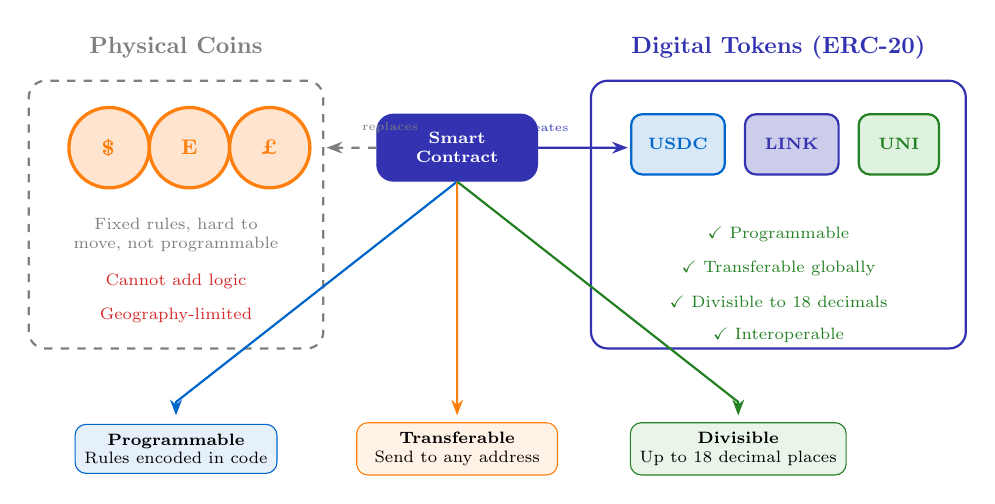
\begin{tikzpicture}[scale=0.85, every node/.style={transform shape}]

% === Left side: Physical Coins ===
\node[font=\normalsize\bfseries, mlgray] at (-5.0,3.5) {Physical Coins};
\draw[mlgray, thick, dashed, rounded corners=6pt] (-7.2,-1.0) rectangle (-2.8,3.0);

% Coin 1
\draw[mlorange, very thick, fill=mlorange!20] (-6.0,2.0) circle (0.6);
\node[font=\small\bfseries, mlorange] at (-6.0,2.0) {\$};
% Coin 2
\draw[mlorange, very thick, fill=mlorange!20] (-4.8,2.0) circle (0.6);
\node[font=\small\bfseries, mlorange] at (-4.8,2.0) {E};
% Coin 3
\draw[mlorange, very thick, fill=mlorange!20] (-3.6,2.0) circle (0.6);
\node[font=\small\bfseries, mlorange] at (-3.6,2.0) {\pounds};

% Limitations
\node[font=\scriptsize, mlgray, text width=3.5cm, align=center] at (-5.0,0.7)
     {Fixed rules, hard to move, not programmable};
\node[font=\scriptsize, mlred] at (-5.0,0.0) {Cannot add logic};
\node[font=\scriptsize, mlred] at (-5.0,-0.5) {Geography-limited};

% === Right side: Digital Tokens ===
\node[font=\normalsize\bfseries, mlpurple] at (4.0,3.5) {Digital Tokens (ERC-20)};
\draw[mlpurple, thick, rounded corners=6pt] (1.2,-1.0) rectangle (6.8,3.0);

% Token rectangles
\draw[mlblue, thick, fill=mlblue!15, rounded corners=4pt] (1.8,1.6) rectangle (3.2,2.5);
\node[font=\scriptsize\bfseries, mlblue] at (2.5,2.05) {USDC};
\draw[mlpurple, thick, fill=mllavender3, rounded corners=4pt] (3.5,1.6) rectangle (4.9,2.5);
\node[font=\scriptsize\bfseries, mlpurple] at (4.2,2.05) {LINK};
\draw[mlgreen!80!black, thick, fill=mlgreen!15, rounded corners=4pt] (5.2,1.6) rectangle (6.4,2.5);
\node[font=\scriptsize\bfseries, mlgreen!80!black] at (5.8,2.05) {UNI};

% Properties
\node[font=\scriptsize, mlgreen!80!black] at (4.0,0.7) {$\checkmark$ Programmable};
\node[font=\scriptsize, mlgreen!80!black] at (4.0,0.2) {$\checkmark$ Transferable globally};
\node[font=\scriptsize, mlgreen!80!black] at (4.0,-0.3) {$\checkmark$ Divisible to 18 decimals};
\node[font=\scriptsize, mlgreen!80!black] at (4.0,-0.8) {$\checkmark$ Interoperable};

% === Center: Smart Contract Node ===
\node[draw=mlpurple, fill=mlpurple, text=white, rounded corners=6pt,
      minimum width=2.4cm, minimum height=1.0cm, font=\scriptsize\bfseries,
      align=center] (sc) at (-0.8,2.0) {Smart\\Contract};

% Arrows from Smart Contract to properties
\draw[-{Stealth[length=2mm]}, mlpurple, thick] (sc.east) -- (1.75,2.0);
\draw[-{Stealth[length=2mm]}, mlgray, thick, dashed] (sc.west) -- (-2.75,2.0);
\node[font=\tiny, mlgray] at (-1.8,2.3) {replaces};
\node[font=\tiny, mlpurple] at (0.5,2.3) {creates};

% === Bottom: Property boxes ===
\node[draw=mlblue, fill=mlblue!10, rounded corners=4pt, font=\scriptsize,
      inner sep=4pt, minimum width=3.0cm, align=center] at (-5.0,-2.5)
     {\textbf{Programmable}\\Rules encoded in code};
\node[draw=mlorange, fill=mlorange!10, rounded corners=4pt, font=\scriptsize,
      inner sep=4pt, minimum width=3.0cm, align=center] at (-0.8,-2.5)
     {\textbf{Transferable}\\Send to any address};
\node[draw=mlgreen!80!black, fill=mlgreen!10, rounded corners=4pt, font=\scriptsize,
      inner sep=4pt, minimum width=3.0cm, align=center] at (3.4,-2.5)
     {\textbf{Divisible}\\Up to 18 decimal places};

% Arrows from smart contract down to property boxes
\draw[-{Stealth[length=2mm]}, mlblue, thick] (sc.south) -- (-5.0,-1.8) -- (-5.0,-2.0);
\draw[-{Stealth[length=2mm]}, mlorange, thick] (sc.south) -- (-0.8,-1.4) -- (-0.8,-2.0);
\draw[-{Stealth[length=2mm]}, mlgreen!80!black, thick] (sc.south) -- (3.4,-1.8) -- (3.4,-2.0);

\end{tikzpicture}
\end{center}

\bottomnote{Tokens are smart contracts that track balances --- they are programmable money.}
\end{frame}

% ==================== FRAME 4: THE ERC-20 STANDARD (Architecture Diagram) ====================
\begin{frame}{The ERC-20 Standard}
\vspace{-2mm}
\begin{center}
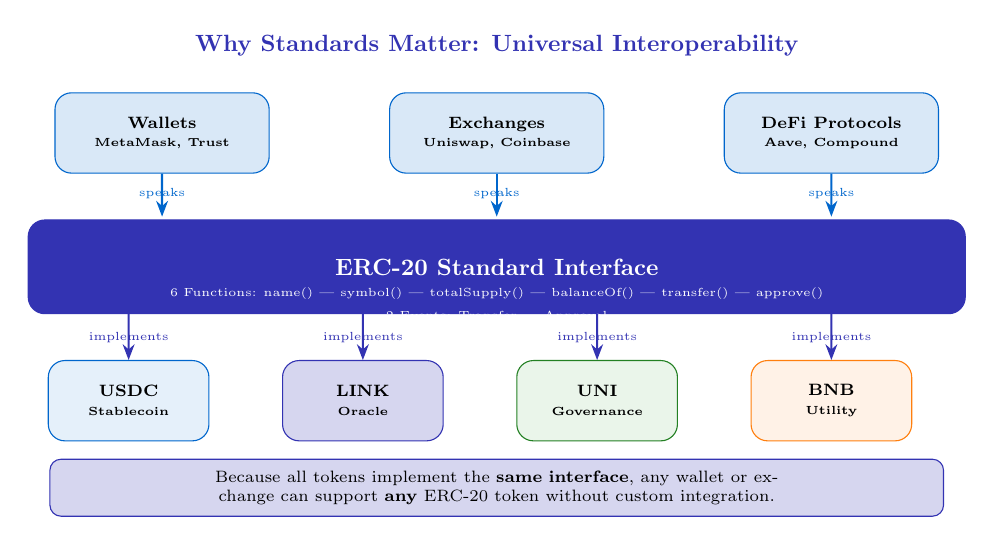
\begin{tikzpicture}[scale=0.85, every node/.style={transform shape}]

% === Top Layer: Consumers ===
\node[font=\normalsize\bfseries, mlpurple] at (0,3.8) {Why Standards Matter: Universal Interoperability};

% Wallet box
\node[draw=mlblue, fill=mlblue!15, rounded corners=6pt,
      minimum width=3.2cm, minimum height=1.2cm, font=\scriptsize\bfseries,
      align=center] (wallet) at (-5.0,2.5) {Wallets\\{\tiny MetaMask, Trust}};

% Exchange box
\node[draw=mlblue, fill=mlblue!15, rounded corners=6pt,
      minimum width=3.2cm, minimum height=1.2cm, font=\scriptsize\bfseries,
      align=center] (exchange) at (0,2.5) {Exchanges\\{\tiny Uniswap, Coinbase}};

% DeFi box
\node[draw=mlblue, fill=mlblue!15, rounded corners=6pt,
      minimum width=3.2cm, minimum height=1.2cm, font=\scriptsize\bfseries,
      align=center] (defi) at (5.0,2.5) {DeFi Protocols\\{\tiny Aave, Compound}};

% === Middle Layer: ERC-20 Standard Interface (wide bar) ===
\node[draw=mlpurple, fill=mlpurple, text=white, rounded corners=6pt,
      minimum width=14.0cm, minimum height=1.4cm, font=\normalsize\bfseries,
      align=center] (standard) at (0,0.5) {ERC-20 Standard Interface};
\node[font=\tiny, white] at (0,0.1) {6 Functions: name() | symbol() | totalSupply() | balanceOf() | transfer() | approve()};
\node[font=\tiny, white] at (0,-0.25) {2 Events: Transfer | Approval};

% Arrows from consumers to standard
\draw[-{Stealth[length=2mm]}, mlblue, thick] (wallet.south) -- (-5.0,1.25);
\draw[-{Stealth[length=2mm]}, mlblue, thick] (exchange.south) -- (0,1.25);
\draw[-{Stealth[length=2mm]}, mlblue, thick] (defi.south) -- (5.0,1.25);

% "speaks" labels
\node[font=\tiny, mlblue] at (-5.0,1.6) {speaks};
\node[font=\tiny, mlblue] at (0,1.6) {speaks};
\node[font=\tiny, mlblue] at (5.0,1.6) {speaks};

% === Bottom Layer: Token Contracts ===
% USDC
\node[draw=mlblue, fill=mlblue!10, rounded corners=6pt,
      minimum width=2.4cm, minimum height=1.2cm, font=\scriptsize\bfseries,
      align=center] (usdc) at (-5.5,-1.5) {USDC\\{\tiny Stablecoin}};

% LINK
\node[draw=mlpurple, fill=mllavender4, rounded corners=6pt,
      minimum width=2.4cm, minimum height=1.2cm, font=\scriptsize\bfseries,
      align=center] (link) at (-2.0,-1.5) {LINK\\{\tiny Oracle}};

% UNI
\node[draw=mlgreen!80!black, fill=mlgreen!10, rounded corners=6pt,
      minimum width=2.4cm, minimum height=1.2cm, font=\scriptsize\bfseries,
      align=center] (uni) at (1.5,-1.5) {UNI\\{\tiny Governance}};

% BNB
\node[draw=mlorange, fill=mlorange!10, rounded corners=6pt,
      minimum width=2.4cm, minimum height=1.2cm, font=\scriptsize\bfseries,
      align=center] (bnb) at (5.0,-1.5) {BNB\\{\tiny Utility}};

% Arrows from standard to tokens
\draw[-{Stealth[length=2mm]}, mlpurple, thick] (-5.5,-0.2) -- (usdc.north);
\draw[-{Stealth[length=2mm]}, mlpurple, thick] (-2.0,-0.2) -- (link.north);
\draw[-{Stealth[length=2mm]}, mlpurple, thick] (1.5,-0.2) -- (uni.north);
\draw[-{Stealth[length=2mm]}, mlpurple, thick] (5.0,-0.2) -- (bnb.north);

% "implements" labels
\node[font=\tiny, mlpurple] at (-5.5,-0.55) {implements};
\node[font=\tiny, mlpurple] at (-2.0,-0.55) {implements};
\node[font=\tiny, mlpurple] at (1.5,-0.55) {implements};
\node[font=\tiny, mlpurple] at (5.0,-0.55) {implements};

% Key insight box at bottom
\node[draw=mlpurple, fill=mllavender4, rounded corners=4pt, font=\scriptsize,
      inner sep=5pt, text width=13cm, align=center] at (0,-2.8)
     {Because all tokens implement the \textbf{same interface}, any wallet or exchange can support \textbf{any} ERC-20 token without custom integration.};

\end{tikzpicture}
\end{center}

\bottomnote{ERC-20 defines 6 functions and 2 events that every fungible token must implement.}
\end{frame}

% ==================== FRAME 5: TRANSFER VS APPROVE (Comic Strip 2) ====================
\begin{frame}{Transfer vs Approve: Two Ways to Move Tokens}
\begin{center}
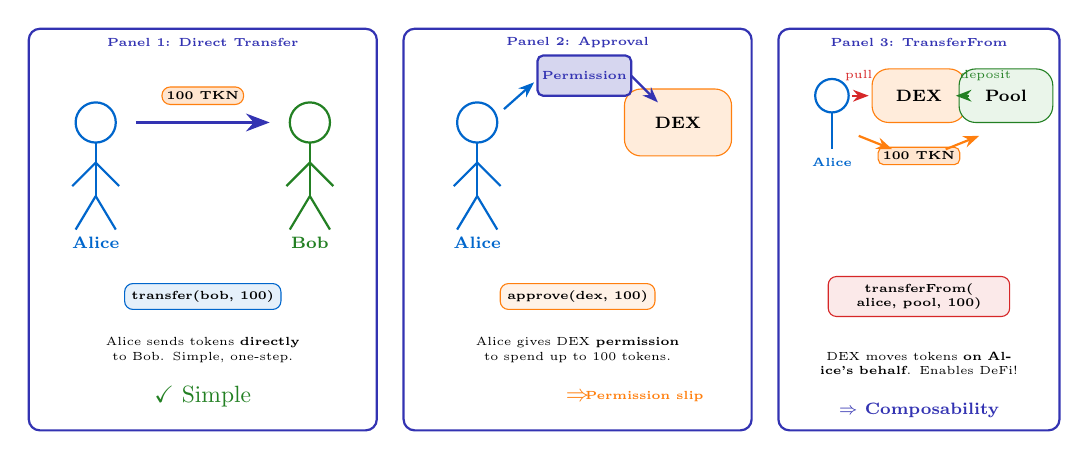
\begin{tikzpicture}[scale=0.85, every node/.style={transform shape}]

% --- Panel 1: Direct Transfer ---
\draw[mlpurple, thick, rounded corners=4pt] (-7.2,-2.8) rectangle (-2.0,3.2);
\node[font=\tiny\bfseries, mlpurple] at (-4.6,3.0) {Panel 1: Direct Transfer};

% Alice stick figure
\draw[mlblue, thick] (-6.2,1.8) circle (0.3);
\draw[mlblue, thick] (-6.2,1.5) -- (-6.2,0.7);
\draw[mlblue, thick] (-6.2,1.2) -- (-6.55,0.85);
\draw[mlblue, thick] (-6.2,1.2) -- (-5.85,0.85);
\draw[mlblue, thick] (-6.2,0.7) -- (-6.5,0.2);
\draw[mlblue, thick] (-6.2,0.7) -- (-5.9,0.2);
\node[font=\scriptsize\bfseries, mlblue] at (-6.2,0.0) {Alice};

% Bob stick figure
\draw[mlgreen!80!black, thick] (-3.0,1.8) circle (0.3);
\draw[mlgreen!80!black, thick] (-3.0,1.5) -- (-3.0,0.7);
\draw[mlgreen!80!black, thick] (-3.0,1.2) -- (-3.35,0.85);
\draw[mlgreen!80!black, thick] (-3.0,1.2) -- (-2.65,0.85);
\draw[mlgreen!80!black, thick] (-3.0,0.7) -- (-3.3,0.2);
\draw[mlgreen!80!black, thick] (-3.0,0.7) -- (-2.7,0.2);
\node[font=\scriptsize\bfseries, mlgreen!80!black] at (-3.0,0.0) {Bob};

% Direct arrow with token
\draw[-{Stealth[length=3mm]}, mlpurple, very thick] (-5.6,1.8) -- (-3.6,1.8);
\node[draw=mlorange, fill=mlorange!20, rounded corners=3pt, font=\tiny\bfseries,
      inner sep=2pt] at (-4.6,2.2) {100 TKN};

% Function label
\node[draw=mlblue, fill=mlblue!10, rounded corners=3pt, font=\tiny\bfseries,
      inner sep=3pt] at (-4.6,-0.8) {transfer(bob, 100)};

% Description
\node[font=\tiny, text width=4.0cm, align=center] at (-4.6,-1.6)
     {Alice sends tokens \textbf{directly} to Bob. Simple, one-step.};

% Checkmark
\node[font=\normalsize, mlgreen!80!black] at (-4.6,-2.3) {$\checkmark$ Simple};

% --- Panel 2: Approval ---
\draw[mlpurple, thick, rounded corners=4pt] (-1.6,-2.8) rectangle (3.6,3.2);
\node[font=\tiny\bfseries, mlpurple] at (1.0,3.0) {Panel 2: Approval};

% Alice stick figure
\draw[mlblue, thick] (-0.5,1.8) circle (0.3);
\draw[mlblue, thick] (-0.5,1.5) -- (-0.5,0.7);
\draw[mlblue, thick] (-0.5,1.2) -- (-0.85,0.85);
\draw[mlblue, thick] (-0.5,1.2) -- (-0.15,0.85);
\draw[mlblue, thick] (-0.5,0.7) -- (-0.8,0.2);
\draw[mlblue, thick] (-0.5,0.7) -- (-0.2,0.2);
\node[font=\scriptsize\bfseries, mlblue] at (-0.5,0.0) {Alice};

% DEX box
\node[draw=mlorange, fill=mlorange!15, rounded corners=6pt,
      minimum width=1.6cm, minimum height=1.0cm, font=\scriptsize\bfseries,
      align=center] (dex1) at (2.5,1.8) {DEX};

% Permission slip
\draw[mlpurple, thick, fill=mllavender4, rounded corners=2pt] (0.4,2.2) rectangle (1.8,2.8);
\node[font=\tiny\bfseries, mlpurple] at (1.1,2.5) {Permission};
\draw[-{Stealth[length=2mm]}, mlpurple, thick] (1.8,2.5) -- (2.2,2.1);

% Arrow from Alice to permission
\draw[-{Stealth[length=2mm]}, mlblue, thick] (-0.1,2.0) -- (0.35,2.4);

% Function label
\node[draw=mlorange, fill=mlorange!10, rounded corners=3pt, font=\tiny\bfseries,
      inner sep=3pt] at (1.0,-0.8) {approve(dex, 100)};

% Description
\node[font=\tiny, text width=4.0cm, align=center] at (1.0,-1.6)
     {Alice gives DEX \textbf{permission} to spend up to 100 tokens.};

% Key icon
\node[font=\normalsize, mlorange] at (1.0,-2.3) {$\Rightarrow$};
\node[font=\tiny\bfseries, mlorange] at (2.0,-2.3) {Permission slip};

% --- Panel 3: TransferFrom ---
\draw[mlpurple, thick, rounded corners=4pt] (4.0,-2.8) rectangle (8.2,3.2);
\node[font=\tiny\bfseries, mlpurple] at (6.1,3.0) {Panel 3: TransferFrom};

% Alice (small, source)
\draw[mlblue, thick] (4.8,2.2) circle (0.25);
\draw[mlblue, thick] (4.8,1.95) -- (4.8,1.4);
\node[font=\tiny\bfseries, mlblue] at (4.8,1.2) {Alice};

% DEX (center, orchestrator)
\node[draw=mlorange, fill=mlorange!15, rounded corners=6pt,
      minimum width=1.4cm, minimum height=0.8cm, font=\scriptsize\bfseries,
      align=center] (dex2) at (6.1,2.2) {DEX};

% Pool (destination)
\node[draw=mlgreen!80!black, fill=mlgreen!10, rounded corners=6pt,
      minimum width=1.4cm, minimum height=0.8cm, font=\scriptsize\bfseries,
      align=center] (pool) at (7.4,2.2) {Pool};

% Arrow: DEX pulls from Alice
\draw[-{Stealth[length=2mm]}, mlred, thick] (5.1,2.2) -- (5.35,2.2);
\node[font=\tiny, mlred] at (5.2,2.5) {pull};

% Arrow: DEX sends to Pool
\draw[-{Stealth[length=2mm]}, mlgreen!80!black, thick] (6.85,2.2) -- (6.65,2.2);
\node[font=\tiny, mlgreen!80!black] at (7.1,2.5) {deposit};

% Token moving
\node[draw=mlorange, fill=mlorange!20, rounded corners=2pt, font=\tiny\bfseries,
      inner sep=2pt] at (6.1,1.3) {100 TKN};
\draw[-{Stealth[length=2mm]}, mlorange, thick] (5.2,1.6) -- (5.7,1.4);
\draw[-{Stealth[length=2mm]}, mlorange, thick] (6.5,1.4) -- (7.0,1.6);

% Function label
\node[draw=mlred, fill=mlred!10, rounded corners=3pt, font=\tiny\bfseries,
      inner sep=3pt, text width=2.5cm, align=center] at (6.1,-0.8) {transferFrom(\\alice, pool, 100)};

% Description
\node[font=\tiny, text width=3.5cm, align=center] at (6.1,-1.8)
     {DEX moves tokens \textbf{on Alice's behalf}. Enables DeFi!};

% Composability note
\node[font=\scriptsize\bfseries, mlpurple] at (6.1,-2.5) {$\Rightarrow$ Composability};

\end{tikzpicture}
\end{center}

\bottomnote{transfer() is for direct sends; approve()+transferFrom() enables DeFi composability.}
\end{frame}

% ==================== FRAME 6: TOKEN SUPPLY MODELS (Visual) ====================
\begin{frame}{Token Supply Models}
\vspace{-2mm}
\begin{center}
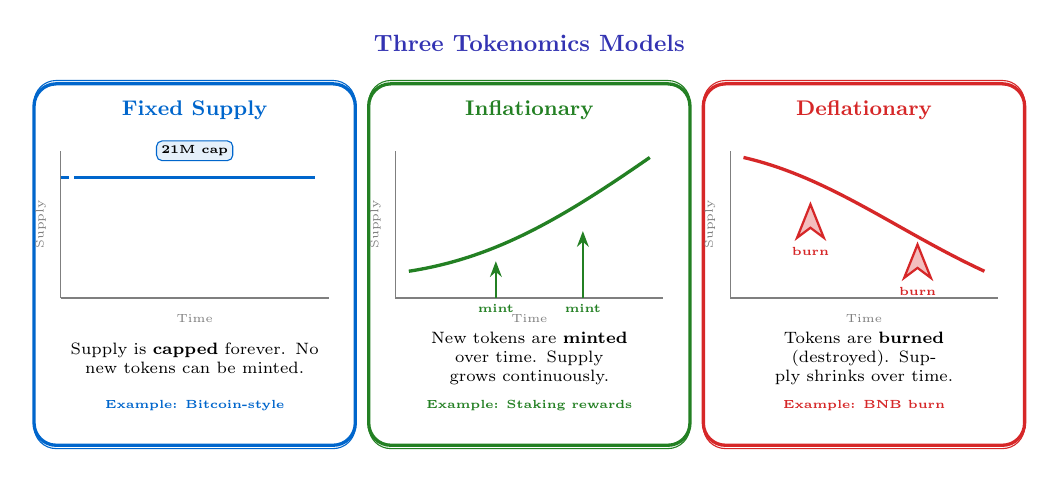
\begin{tikzpicture}[scale=0.85, every node/.style={transform shape}]

\node[font=\normalsize\bfseries, mlpurple] at (0,3.8) {Three Tokenomics Models};

% === Model 1: Fixed Supply ===
\node[draw=mlblue, fill=white, rounded corners=8pt, minimum width=4.8cm,
      minimum height=5.5cm, inner sep=5pt] at (-5.0,0.5) {};
\draw[mlblue, very thick, rounded corners=8pt] (-7.4,-2.2) rectangle (-2.6,3.2);

\node[font=\small\bfseries, mlblue] at (-5.0,2.8) {Fixed Supply};

% Flat horizontal line
\draw[mlgray, thin] (-7.0,0.0) -- (-3.0,0.0); % x-axis
\draw[mlgray, thin] (-7.0,0.0) -- (-7.0,2.2); % y-axis
\node[font=\tiny, mlgray] at (-7.3,1.1) {\rotatebox{90}{Supply}};
\node[font=\tiny, mlgray] at (-5.0,-0.3) {Time};

% Flat supply line with cap
\draw[mlblue, very thick] (-6.8,1.8) -- (-3.2,1.8);
\draw[mlblue, thick, dashed] (-7.0,1.8) -- (-6.8,1.8);

% Cap label
\node[draw=mlblue, fill=mlblue!10, rounded corners=2pt, font=\tiny\bfseries,
      inner sep=2pt] at (-5.0,2.2) {21M cap};

% Description
\node[font=\scriptsize, text width=3.8cm, align=center] at (-5.0,-0.9)
     {Supply is \textbf{capped} forever. No new tokens can be minted.};
\node[font=\tiny\bfseries, mlblue] at (-5.0,-1.6) {Example: Bitcoin-style};

% === Model 2: Inflationary ===
\node[draw=mlgreen!80!black, fill=white, rounded corners=8pt, minimum width=4.8cm,
      minimum height=5.5cm, inner sep=5pt] at (0,0.5) {};
\draw[mlgreen!80!black, very thick, rounded corners=8pt] (-2.4,-2.2) rectangle (2.4,3.2);

\node[font=\small\bfseries, mlgreen!80!black] at (0,2.8) {Inflationary};

% Upward curve
\draw[mlgray, thin] (-2.0,0.0) -- (2.0,0.0); % x-axis
\draw[mlgray, thin] (-2.0,0.0) -- (-2.0,2.2); % y-axis
\node[font=\tiny, mlgray] at (-2.3,1.1) {\rotatebox{90}{Supply}};
\node[font=\tiny, mlgray] at (0,-0.3) {Time};

% Upward curve
\draw[mlgreen!80!black, very thick] (-1.8,0.4) .. controls (-0.5,0.6) and (0.5,1.2) .. (1.8,2.1);

% Mint arrows (pointing up into curve)
\draw[-{Stealth[length=2mm]}, mlgreen!80!black, thick] (-0.5,0.0) -- (-0.5,0.55);
\node[font=\tiny\bfseries, mlgreen!80!black] at (-0.5,-0.15) {mint};
\draw[-{Stealth[length=2mm]}, mlgreen!80!black, thick] (0.8,0.0) -- (0.8,1.0);
\node[font=\tiny\bfseries, mlgreen!80!black] at (0.8,-0.15) {mint};

% Description
\node[font=\scriptsize, text width=3.8cm, align=center] at (0,-0.9)
     {New tokens are \textbf{minted} over time. Supply grows continuously.};
\node[font=\tiny\bfseries, mlgreen!80!black] at (0,-1.6) {Example: Staking rewards};

% === Model 3: Deflationary ===
\node[draw=mlred, fill=white, rounded corners=8pt, minimum width=4.8cm,
      minimum height=5.5cm, inner sep=5pt] at (5.0,0.5) {};
\draw[mlred, very thick, rounded corners=8pt] (2.6,-2.2) rectangle (7.4,3.2);

\node[font=\small\bfseries, mlred] at (5.0,2.8) {Deflationary};

% Downward curve
\draw[mlgray, thin] (3.0,0.0) -- (7.0,0.0); % x-axis
\draw[mlgray, thin] (3.0,0.0) -- (3.0,2.2); % y-axis
\node[font=\tiny, mlgray] at (2.7,1.1) {\rotatebox{90}{Supply}};
\node[font=\tiny, mlgray] at (5.0,-0.3) {Time};

% Downward curve
\draw[mlred, very thick] (3.2,2.1) .. controls (4.5,1.8) and (5.5,1.0) .. (6.8,0.4);

% Burn flames (pointing down from curve)
\draw[mlred, thick, fill=mlred!30] (4.2,1.4) -- (4.0,0.9) -- (4.2,1.05) -- (4.4,0.9) -- cycle;
\node[font=\tiny\bfseries, mlred] at (4.2,0.7) {burn};
\draw[mlred, thick, fill=mlred!30] (5.8,0.8) -- (5.6,0.3) -- (5.8,0.45) -- (6.0,0.3) -- cycle;
\node[font=\tiny\bfseries, mlred] at (5.8,0.1) {burn};

% Description
\node[font=\scriptsize, text width=3.8cm, align=center] at (5.0,-0.9)
     {Tokens are \textbf{burned} (destroyed). Supply shrinks over time.};
\node[font=\tiny\bfseries, mlred] at (5.0,-1.6) {Example: BNB burn};

\end{tikzpicture}
\end{center}

\bottomnote{Token economics (tokenomics) determine long-term value and sustainability.}
\end{frame}

% ==================== FRAME 7: BUILDING YOUR TOKEN (Flow Diagram) ====================
\begin{frame}{Building Your Token}
\vspace{-2mm}
\begin{center}
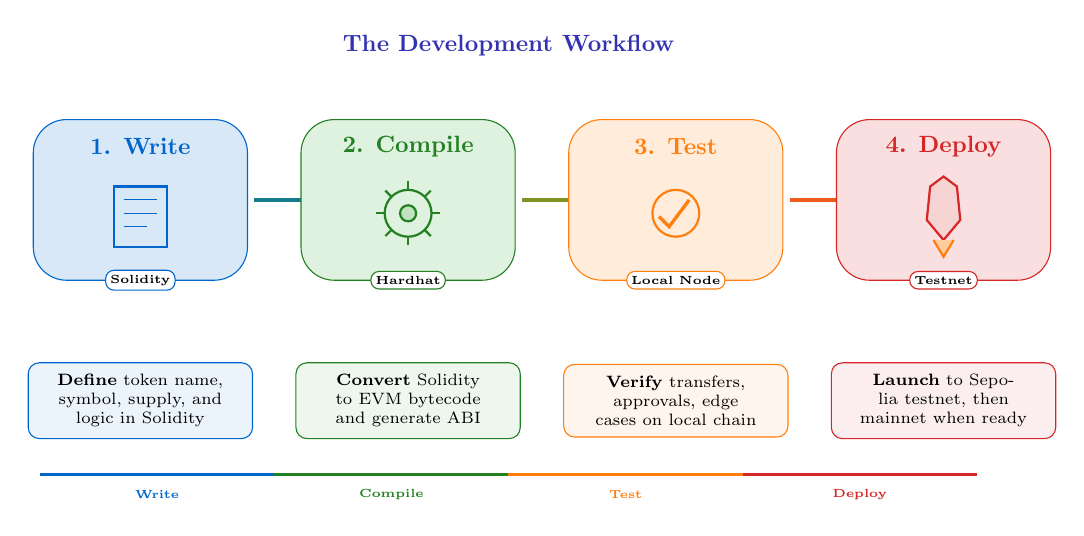
\begin{tikzpicture}[scale=0.85, every node/.style={transform shape}]

\node[font=\normalsize\bfseries, mlpurple] at (0,3.8) {The Development Workflow};

% === Step 1: Write ===
\node[draw=mlblue, fill=mlblue!15, rounded corners=12pt,
      minimum width=3.2cm, minimum height=2.4cm, inner sep=5pt]
      (write) at (-5.5,1.5) {};
\node[font=\normalsize\bfseries, mlblue] at (-5.5,2.3) {1. Write};

% Document icon
\draw[mlblue, thick] (-5.9,0.8) rectangle (-5.1,1.7);
\draw[mlblue, thin] (-5.75,1.5) -- (-5.25,1.5);
\draw[mlblue, thin] (-5.75,1.3) -- (-5.25,1.3);
\draw[mlblue, thin] (-5.75,1.1) -- (-5.4,1.1);

% Tool label
\node[draw=mlblue, fill=white, rounded corners=3pt, font=\tiny\bfseries,
      inner sep=2pt] at (-5.5,0.3) {Solidity};

% Arrow 1 -> 2
\draw[-{Stealth[length=4mm]}, mlblue!60!mlgreen, very thick] (-3.8,1.5) -- (-2.6,1.5);

% === Step 2: Compile ===
\node[draw=mlgreen!80!black, fill=mlgreen!15, rounded corners=12pt,
      minimum width=3.2cm, minimum height=2.4cm, inner sep=5pt]
      (compile) at (-1.5,1.5) {};
\node[font=\normalsize\bfseries, mlgreen!80!black] at (-1.5,2.3) {2. Compile};

% Gear icon
\draw[mlgreen!80!black, thick] (-1.5,1.3) circle (0.35);
\foreach \angle in {0,45,90,135,180,225,270,315} {
    \draw[mlgreen!80!black, thick] ($(-1.5,1.3)+(\angle:0.35)$) -- ($(-1.5,1.3)+(\angle:0.48)$);
}
\draw[mlgreen!80!black, thick, fill=mlgreen!30] (-1.5,1.3) circle (0.12);

% Tool label
\node[draw=mlgreen!80!black, fill=white, rounded corners=3pt, font=\tiny\bfseries,
      inner sep=2pt] at (-1.5,0.3) {Hardhat};

% Arrow 2 -> 3
\draw[-{Stealth[length=4mm]}, mlgreen!60!mlorange, very thick] (0.2,1.5) -- (1.4,1.5);

% === Step 3: Test ===
\node[draw=mlorange, fill=mlorange!15, rounded corners=12pt,
      minimum width=3.2cm, minimum height=2.4cm, inner sep=5pt]
      (test) at (2.5,1.5) {};
\node[font=\normalsize\bfseries, mlorange] at (2.5,2.3) {3. Test};

% Checkmark in circle
\draw[mlorange, thick] (2.5,1.3) circle (0.35);
\draw[mlorange, very thick] (2.25,1.25) -- (2.4,1.1) -- (2.7,1.5);

% Tool label
\node[draw=mlorange, fill=white, rounded corners=3pt, font=\tiny\bfseries,
      inner sep=2pt] at (2.5,0.3) {Local Node};

% Arrow 3 -> 4
\draw[-{Stealth[length=4mm]}, mlorange!60!mlred, very thick] (4.2,1.5) -- (5.4,1.5);

% === Step 4: Deploy ===
\node[draw=mlred, fill=mlred!15, rounded corners=12pt,
      minimum width=3.2cm, minimum height=2.4cm, inner sep=5pt]
      (deploy) at (6.5,1.5) {};
\node[font=\normalsize\bfseries, mlred] at (6.5,2.3) {4. Deploy};

% Rocket icon
\draw[mlred, thick, fill=mlred!20] (6.5,0.9) -- (6.25,1.2) -- (6.3,1.7) --
     (6.5,1.85) -- (6.7,1.7) -- (6.75,1.2) -- cycle;
\draw[mlorange, thick, fill=mlorange!40] (6.35,0.9) -- (6.5,0.65) -- (6.65,0.9);

% Tool label
\node[draw=mlred, fill=white, rounded corners=3pt, font=\tiny\bfseries,
      inner sep=2pt] at (6.5,0.3) {Testnet};

% === Bottom detail boxes ===
\node[draw=mlblue, fill=mlblue!8, rounded corners=4pt, font=\scriptsize,
      inner sep=5pt, text width=3.0cm, align=center] at (-5.5,-1.5)
     {\textbf{Define} token name, symbol, supply, and logic in Solidity};

\node[draw=mlgreen!80!black, fill=mlgreen!8, rounded corners=4pt, font=\scriptsize,
      inner sep=5pt, text width=3.0cm, align=center] at (-1.5,-1.5)
     {\textbf{Convert} Solidity to EVM bytecode and generate ABI};

\node[draw=mlorange, fill=mlorange!8, rounded corners=4pt, font=\scriptsize,
      inner sep=5pt, text width=3.0cm, align=center] at (2.5,-1.5)
     {\textbf{Verify} transfers, approvals, edge cases on local chain};

\node[draw=mlred, fill=mlred!8, rounded corners=4pt, font=\scriptsize,
      inner sep=5pt, text width=3.0cm, align=center] at (6.5,-1.5)
     {\textbf{Launch} to Sepolia testnet, then mainnet when ready};

% Color progression bar at very bottom
\draw[mlblue, very thick] (-7.0,-2.6) -- (-3.5,-2.6);
\draw[mlgreen!80!black, very thick] (-3.5,-2.6) -- (0,-2.6);
\draw[mlorange, very thick] (0,-2.6) -- (3.5,-2.6);
\draw[mlred, very thick] (3.5,-2.6) -- (7.0,-2.6);
\node[font=\tiny\bfseries, mlblue] at (-5.25,-2.9) {Write};
\node[font=\tiny\bfseries, mlgreen!80!black] at (-1.75,-2.9) {Compile};
\node[font=\tiny\bfseries, mlorange] at (1.75,-2.9) {Test};
\node[font=\tiny\bfseries, mlred] at (5.25,-2.9) {Deploy};

\end{tikzpicture}
\end{center}

\bottomnote{The development workflow follows: write, compile, test locally, deploy to testnet.}
\end{frame}

% ==================== FRAME 8: REAL TOKENS IN THE WILD (Data Snapshot) ====================
\begin{frame}{Real Tokens in the Wild}
\vspace{-2mm}
\begin{center}
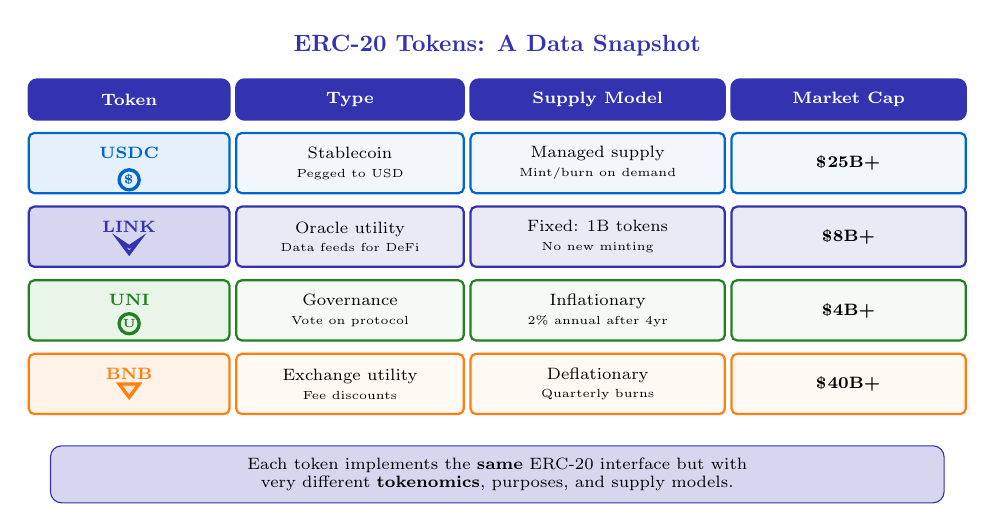
\begin{tikzpicture}[scale=0.85, every node/.style={transform shape}]

\node[font=\normalsize\bfseries, mlpurple] at (0,3.8) {ERC-20 Tokens: A Data Snapshot};

% === Header Row ===
\draw[mlpurple, thick, fill=mlpurple, rounded corners=3pt] (-7.0,2.7) rectangle (-4.0,3.3);
\node[font=\scriptsize\bfseries, white] at (-5.5,3.0) {Token};

\draw[mlpurple, thick, fill=mlpurple, rounded corners=3pt] (-3.9,2.7) rectangle (-0.5,3.3);
\node[font=\scriptsize\bfseries, white] at (-2.2,3.0) {Type};

\draw[mlpurple, thick, fill=mlpurple, rounded corners=3pt] (-0.4,2.7) rectangle (3.4,3.3);
\node[font=\scriptsize\bfseries, white] at (1.5,3.0) {Supply Model};

\draw[mlpurple, thick, fill=mlpurple, rounded corners=3pt] (3.5,2.7) rectangle (7.0,3.3);
\node[font=\scriptsize\bfseries, white] at (5.25,3.0) {Market Cap};

% === Row 1: USDC ===
\draw[mlblue, thick, fill=mlblue!10, rounded corners=2pt] (-7.0,1.6) rectangle (-4.0,2.5);
\node[font=\scriptsize\bfseries, mlblue] at (-5.5,2.2) {USDC};
\draw[mlblue, very thick] (-5.5,1.8) circle (0.15);
\node[font=\tiny\bfseries, mlblue] at (-5.5,1.8) {\$};

\draw[mlblue, thick, fill=mlblue!5, rounded corners=2pt] (-3.9,1.6) rectangle (-0.5,2.5);
\node[font=\scriptsize, align=center] at (-2.2,2.05) {Stablecoin\\{\tiny Pegged to USD}};

\draw[mlblue, thick, fill=mlblue!5, rounded corners=2pt] (-0.4,1.6) rectangle (3.4,2.5);
\node[font=\scriptsize, align=center] at (1.5,2.05) {Managed supply\\{\tiny Mint/burn on demand}};

\draw[mlblue, thick, fill=mlblue!5, rounded corners=2pt] (3.5,1.6) rectangle (7.0,2.5);
\node[font=\scriptsize\bfseries] at (5.25,2.05) {\$25B+};

% === Row 2: LINK ===
\draw[mlpurple, thick, fill=mllavender4, rounded corners=2pt] (-7.0,0.5) rectangle (-4.0,1.4);
\node[font=\scriptsize\bfseries, mlpurple] at (-5.5,1.1) {LINK};
\draw[mlpurple, very thick, fill=mllavender3] (-5.5,0.7) -- (-5.35,0.9) -- (-5.5,0.8) -- (-5.65,0.9) -- cycle;

\draw[mlpurple, thick, fill=mllavender4!50, rounded corners=2pt] (-3.9,0.5) rectangle (-0.5,1.4);
\node[font=\scriptsize, align=center] at (-2.2,0.95) {Oracle utility\\{\tiny Data feeds for DeFi}};

\draw[mlpurple, thick, fill=mllavender4!50, rounded corners=2pt] (-0.4,0.5) rectangle (3.4,1.4);
\node[font=\scriptsize, align=center] at (1.5,0.95) {Fixed: 1B tokens\\{\tiny No new minting}};

\draw[mlpurple, thick, fill=mllavender4!50, rounded corners=2pt] (3.5,0.5) rectangle (7.0,1.4);
\node[font=\scriptsize\bfseries] at (5.25,0.95) {\$8B+};

% === Row 3: UNI ===
\draw[mlgreen!80!black, thick, fill=mlgreen!10, rounded corners=2pt] (-7.0,-0.6) rectangle (-4.0,0.3);
\node[font=\scriptsize\bfseries, mlgreen!80!black] at (-5.5,-0.0) {UNI};
\draw[mlgreen!80!black, very thick] (-5.5,-0.35) circle (0.15);
\node[font=\tiny\bfseries, mlgreen!80!black] at (-5.5,-0.35) {U};

\draw[mlgreen!80!black, thick, fill=mlgreen!5, rounded corners=2pt] (-3.9,-0.6) rectangle (-0.5,0.3);
\node[font=\scriptsize, align=center] at (-2.2,-0.15) {Governance\\{\tiny Vote on protocol}};

\draw[mlgreen!80!black, thick, fill=mlgreen!5, rounded corners=2pt] (-0.4,-0.6) rectangle (3.4,0.3);
\node[font=\scriptsize, align=center] at (1.5,-0.15) {Inflationary\\{\tiny 2\% annual after 4yr}};

\draw[mlgreen!80!black, thick, fill=mlgreen!5, rounded corners=2pt] (3.5,-0.6) rectangle (7.0,0.3);
\node[font=\scriptsize\bfseries] at (5.25,-0.15) {\$4B+};

% === Row 4: BNB ===
\draw[mlorange, thick, fill=mlorange!10, rounded corners=2pt] (-7.0,-1.7) rectangle (-4.0,-0.8);
\node[font=\scriptsize\bfseries, mlorange] at (-5.5,-1.1) {BNB};
\draw[mlorange, very thick, fill=mlorange!20] (-5.5,-1.45) -- (-5.35,-1.25) -- (-5.65,-1.25) -- cycle;

\draw[mlorange, thick, fill=mlorange!5, rounded corners=2pt] (-3.9,-1.7) rectangle (-0.5,-0.8);
\node[font=\scriptsize, align=center] at (-2.2,-1.25) {Exchange utility\\{\tiny Fee discounts}};

\draw[mlorange, thick, fill=mlorange!5, rounded corners=2pt] (-0.4,-1.7) rectangle (3.4,-0.8);
\node[font=\scriptsize, align=center] at (1.5,-1.25) {Deflationary\\{\tiny Quarterly burns}};

\draw[mlorange, thick, fill=mlorange!5, rounded corners=2pt] (3.5,-1.7) rectangle (7.0,-0.8);
\node[font=\scriptsize\bfseries] at (5.25,-1.25) {\$40B+};

% === Summary bar ===
\node[draw=mlpurple, fill=mllavender4, rounded corners=4pt, font=\scriptsize,
      inner sep=5pt, text width=13cm, align=center] at (0,-2.6)
     {Each token implements the \textbf{same} ERC-20 interface but with very different \textbf{tokenomics}, purposes, and supply models.};

\end{tikzpicture}
\end{center}

\bottomnote{Over 500,000 ERC-20 tokens exist on Ethereum alone.}
\end{frame}

% ==================== FRAME 9: SECURITY --- THE FINE PRINT (Comic Strip 3) ====================
\begin{frame}{Security --- The Fine Print}
\begin{center}
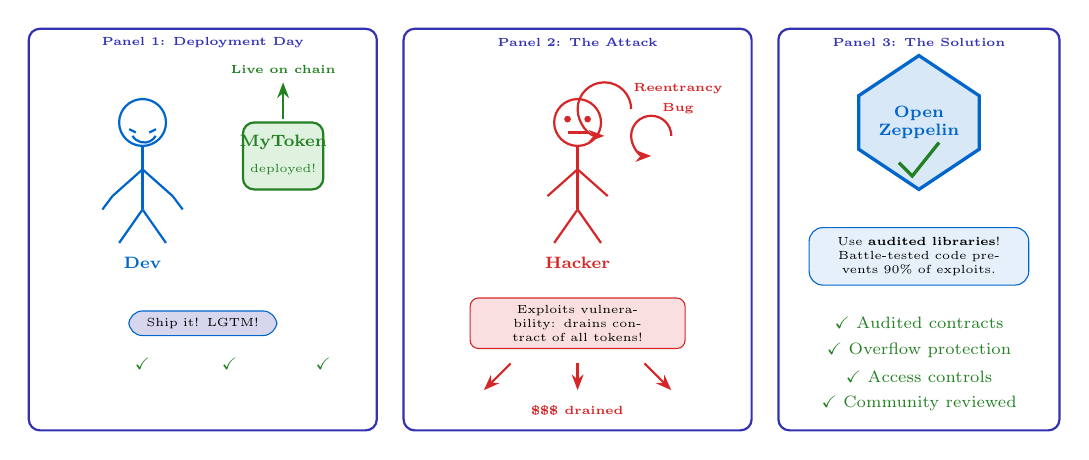
\begin{tikzpicture}[scale=0.85, every node/.style={transform shape}]

% --- Panel 1: Happy deployment ---
\draw[mlpurple, thick, rounded corners=4pt] (-7.2,-2.8) rectangle (-2.0,3.2);
\node[font=\tiny\bfseries, mlpurple] at (-4.6,3.0) {Panel 1: Deployment Day};

% Developer stick figure (happy)
\draw[mlblue, thick] (-5.5,1.8) circle (0.35);
\draw[mlblue, thick] (-5.5,1.45) -- (-5.5,0.5);
\draw[mlblue, thick] (-5.5,1.1) -- (-5.95,0.7);
\draw[mlblue, thick] (-5.5,1.1) -- (-5.05,0.7);
\draw[mlblue, thick] (-5.5,0.5) -- (-5.85,0.0);
\draw[mlblue, thick] (-5.5,0.5) -- (-5.15,0.0);
\node[font=\scriptsize\bfseries, mlblue] at (-5.5,-0.3) {Dev};

% Smile
\draw[mlblue, thick] (-5.7,1.7) -- (-5.6,1.65);
\draw[mlblue, thick] (-5.3,1.7) -- (-5.4,1.65);
\draw[mlblue, thick] (-5.65,1.6) arc (210:330:0.2);

% Raised arms (celebration)
\draw[mlblue, thick] (-5.95,0.7) -- (-6.1,0.5);
\draw[mlblue, thick] (-5.05,0.7) -- (-4.9,0.5);

% Contract deploying (rocket effect)
\draw[mlgreen!80!black, thick, fill=mlgreen!15, rounded corners=4pt]
     (-4.0,0.8) rectangle (-2.8,1.8);
\node[font=\scriptsize\bfseries, mlgreen!80!black] at (-3.4,1.5) {MyToken};
\node[font=\tiny, mlgreen!80!black] at (-3.4,1.1) {deployed!};

% Upward arrow
\draw[-{Stealth[length=2mm]}, mlgreen!80!black, thick] (-3.4,1.85) -- (-3.4,2.4);
\node[font=\tiny\bfseries, mlgreen!80!black] at (-3.4,2.6) {Live on chain};

% Speech bubble
\node[draw=mlblue, fill=mllavender4, rounded corners=5pt, font=\tiny,
      text width=2.0cm, align=center, inner sep=3pt]
      at (-4.6,-1.2) {Ship it! LGTM!};

% Party indicators
\node[font=\scriptsize, mlgreen!80!black] at (-5.5,-1.8) {$\checkmark$};
\node[font=\scriptsize, mlgreen!80!black] at (-4.2,-1.8) {$\checkmark$};
\node[font=\scriptsize, mlgreen!80!black] at (-2.8,-1.8) {$\checkmark$};

% --- Panel 2: Hacker finds exploit ---
\draw[mlpurple, thick, rounded corners=4pt] (-1.6,-2.8) rectangle (3.6,3.2);
\node[font=\tiny\bfseries, mlpurple] at (1.0,3.0) {Panel 2: The Attack};

% Hacker stick figure
\draw[mlred, thick] (1.0,1.8) circle (0.35);
\draw[mlred, thick] (1.0,1.45) -- (1.0,0.5);
\draw[mlred, thick] (1.0,1.1) -- (0.55,0.7);
\draw[mlred, thick] (1.0,1.1) -- (1.45,0.7);
\draw[mlred, thick] (1.0,0.5) -- (0.65,0.0);
\draw[mlred, thick] (1.0,0.5) -- (1.35,0.0);
\node[font=\scriptsize\bfseries, mlred] at (1.0,-0.3) {Hacker};

% Evil eyes
\fill[mlred] (0.85,1.85) circle (0.05);
\fill[mlred] (1.15,1.85) circle (0.05);
% Grin
\draw[mlred, thick] (0.85,1.65) -- (1.15,1.65);

% Reentrancy arrows (going in circles)
\draw[mlred, thick, -{Stealth[length=2mm]}] (1.8,2.0) arc (0:270:0.4);
\draw[mlred, thick, -{Stealth[length=2mm]}] (2.4,1.6) arc (0:270:0.3);
\node[font=\tiny\bfseries, mlred] at (2.5,2.3) {Reentrancy};
\node[font=\tiny\bfseries, mlred] at (2.5,2.0) {Bug};

% Stolen funds
\node[draw=mlred, fill=mlred!15, rounded corners=3pt, font=\tiny,
      text width=3.0cm, align=center, inner sep=3pt]
      at (1.0,-1.2) {Exploits vulnerability: drains contract of all tokens!};

% Money draining
\draw[-{Stealth[length=2mm]}, mlred, thick] (0.0,-1.8) -- (-0.4,-2.2);
\draw[-{Stealth[length=2mm]}, mlred, thick] (1.0,-1.8) -- (1.0,-2.2);
\draw[-{Stealth[length=2mm]}, mlred, thick] (2.0,-1.8) -- (2.4,-2.2);
\node[font=\tiny\bfseries, mlred] at (1.0,-2.5) {\$\$\$ drained};

% --- Panel 3: OpenZeppelin to the rescue ---
\draw[mlpurple, thick, rounded corners=4pt] (4.0,-2.8) rectangle (8.2,3.2);
\node[font=\tiny\bfseries, mlpurple] at (6.1,3.0) {Panel 3: The Solution};

% Shield (OpenZeppelin)
\draw[mlblue, very thick, fill=mlblue!15]
     (6.1,0.8) -- (5.2,1.4) -- (5.2,2.2) -- (6.1,2.8) -- (7.0,2.2) -- (7.0,1.4) -- cycle;
\node[font=\scriptsize\bfseries, mlblue, text width=1.5cm, align=center] at (6.1,1.8) {Open\\Zeppelin};

% Checkmark on shield
\draw[mlgreen!80!black, very thick] (5.8,1.2) -- (6.0,1.0) -- (6.4,1.5);

% Speech bubble
\node[draw=mlblue, fill=mlblue!10, rounded corners=5pt, font=\tiny,
      text width=3.0cm, align=center, inner sep=4pt]
      at (6.1,-0.2) {Use \textbf{audited libraries}! Battle-tested code prevents 90\% of exploits.};

% Security checklist
\node[font=\scriptsize, mlgreen!80!black] at (6.1,-1.2) {$\checkmark$ Audited contracts};
\node[font=\scriptsize, mlgreen!80!black] at (6.1,-1.6) {$\checkmark$ Overflow protection};
\node[font=\scriptsize, mlgreen!80!black] at (6.1,-2.0) {$\checkmark$ Access controls};
\node[font=\scriptsize, mlgreen!80!black] at (6.1,-2.4) {$\checkmark$ Community reviewed};

\end{tikzpicture}
\end{center}

\bottomnote{Smart contract bugs are permanent --- use OpenZeppelin and get audits before mainnet.}
\end{frame}

% ==================== FRAME 10: KEY TAKEAWAYS ====================
\begin{frame}{Key Takeaways}
\vspace{-2mm}
\begin{center}
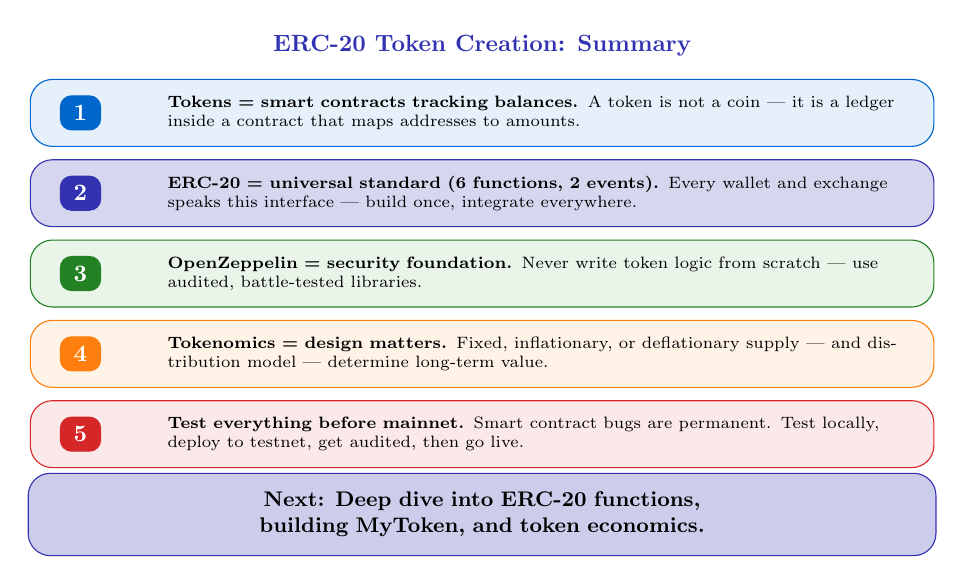
\begin{tikzpicture}[scale=0.85, every node/.style={transform shape}]

\node[font=\normalsize\bfseries, mlpurple] at (0,3.8) {ERC-20 Token Creation: Summary};

% === Takeaway 1 ===
\node[draw=mlblue, fill=mlblue!10, rounded corners=8pt,
      minimum width=13.5cm, minimum height=1.0cm, inner sep=5pt]
      (t1) at (0,2.8) {};
\node[draw=mlblue, fill=mlblue, text=white, rounded corners=4pt,
      font=\normalsize\bfseries, inner sep=4pt, minimum width=0.6cm]
      at (-6.0,2.8) {1};
\node[font=\scriptsize, text width=11.0cm, align=left] at (0.8,2.8)
     {\textbf{Tokens = smart contracts tracking balances.} A token is not a coin --- it is a ledger inside a contract that maps addresses to amounts.};

% === Takeaway 2 ===
\node[draw=mlpurple, fill=mllavender4, rounded corners=8pt,
      minimum width=13.5cm, minimum height=1.0cm, inner sep=5pt]
      (t2) at (0,1.6) {};
\node[draw=mlpurple, fill=mlpurple, text=white, rounded corners=4pt,
      font=\normalsize\bfseries, inner sep=4pt, minimum width=0.6cm]
      at (-6.0,1.6) {2};
\node[font=\scriptsize, text width=11.0cm, align=left] at (0.8,1.6)
     {\textbf{ERC-20 = universal standard (6 functions, 2 events).} Every wallet and exchange speaks this interface --- build once, integrate everywhere.};

% === Takeaway 3 ===
\node[draw=mlgreen!80!black, fill=mlgreen!10, rounded corners=8pt,
      minimum width=13.5cm, minimum height=1.0cm, inner sep=5pt]
      (t3) at (0,0.4) {};
\node[draw=mlgreen!80!black, fill=mlgreen!80!black, text=white, rounded corners=4pt,
      font=\normalsize\bfseries, inner sep=4pt, minimum width=0.6cm]
      at (-6.0,0.4) {3};
\node[font=\scriptsize, text width=11.0cm, align=left] at (0.8,0.4)
     {\textbf{OpenZeppelin = security foundation.} Never write token logic from scratch --- use audited, battle-tested libraries.};

% === Takeaway 4 ===
\node[draw=mlorange, fill=mlorange!10, rounded corners=8pt,
      minimum width=13.5cm, minimum height=1.0cm, inner sep=5pt]
      (t4) at (0,-0.8) {};
\node[draw=mlorange, fill=mlorange, text=white, rounded corners=4pt,
      font=\normalsize\bfseries, inner sep=4pt, minimum width=0.6cm]
      at (-6.0,-0.8) {4};
\node[font=\scriptsize, text width=11.0cm, align=left] at (0.8,-0.8)
     {\textbf{Tokenomics = design matters.} Fixed, inflationary, or deflationary supply --- and distribution model --- determine long-term value.};

% === Takeaway 5 ===
\node[draw=mlred, fill=mlred!10, rounded corners=8pt,
      minimum width=13.5cm, minimum height=1.0cm, inner sep=5pt]
      (t5) at (0,-2.0) {};
\node[draw=mlred, fill=mlred, text=white, rounded corners=4pt,
      font=\normalsize\bfseries, inner sep=4pt, minimum width=0.6cm]
      at (-6.0,-2.0) {5};
\node[font=\scriptsize, text width=11.0cm, align=left] at (0.8,-2.0)
     {\textbf{Test everything before mainnet.} Smart contract bugs are permanent. Test locally, deploy to testnet, get audited, then go live.};

% === Next lecture teaser ===
\node[draw=mlpurple, fill=mllavender3, rounded corners=8pt,
      font=\small, inner sep=8pt, text width=13cm, align=center]
      at (0,-3.2) {\textbf{Next: Deep dive into ERC-20 functions, building MyToken, and token economics.}};

\end{tikzpicture}
\end{center}

\bottomnote{Next: Deep dive into ERC-20 functions, building MyToken, and token economics.}
\end{frame}

\end{document}
